\subsection{Binning and selection optimization}\label{sec:binopt}
\emph{Note that the numbers in this subsection are upper limits on the \tHq+\tHW\ cross sections only (without \ttH), and are always evaluated at $\Ct=-1.0$, $\CV=1.0$.}
\hrule

The effect on the cross section limit of the choice of pre-selection cuts is evaluated by varying the most important cuts and re-calculating the limit (in the three lepton channel) in each case.
Table~\ref{cut_limit} shows the several variations made, compared to a baseline corresponding to the selection reported in Tab.~\ref{tab:evsel}, but with only a loose CSV jet and a \Z\ veto of $\pm10\GeV$.
The optimal limit is found when requiring a slightly tighter selection with respect to the baseline.
This is the selection reported in Tab.~\ref{tab:evsel}.

\begin{table}[h!]
\centering
\begin{tabular}{lll}
Selection                         & Variation                & Expected limit \\ \hline
Baseline                          & see Tab.~\ref{tab:evsel} & $<2.93$\\
Loose CSV tags                    & $\geq 1 \to \geq 2$      & $<3.81$\\
Medium CSV tags                   & $\geq 0 \to \geq 1$      & $<2.76$\\
Light forward jet $\eta$          & $\geq 0 \to \geq 1$      & $<2.94$\\
Light forward jet $\eta$          & $\geq 0 \to \geq 1.5$    & $<3.00$\\
$\MET>30\GeV$                     &                          & $<2.91$\\
\Z\ veto ($|m_{\ell\ell}-m_\Z|$)  & $>10\GeV \to >15\GeV$    & $<2.79$\\
One medium CSV + 15\GeV\ \Z\ veto & combined                 & $<2.62$\\\hline
\end{tabular}
\caption{Limit variation as a function of tighter cuts. The baseline selection corresponds to a looser selection as the one reported in Tab.~\ref{tab:evsel} (which is the optimal selection determined here (last line)), where only a CSV-loose \cPqb-tagged jet is required, and the \Z\ veto is loosened to $\pm10\GeV$.}
\label{cut_limit}
\end{table}

The obtained cross section limit also depends on the chosen binning in the 2D plane as the S/B ratio varies across the plane, hence several sizes and binning combination were tested in order to optimize the limit.
Figure~\ref{bins} show some of the binning combinations tested; in the default combination all the bins have the same size, while the best limit was found for a set of 10 bins.

\begin{figure} [!h]
 \centering
 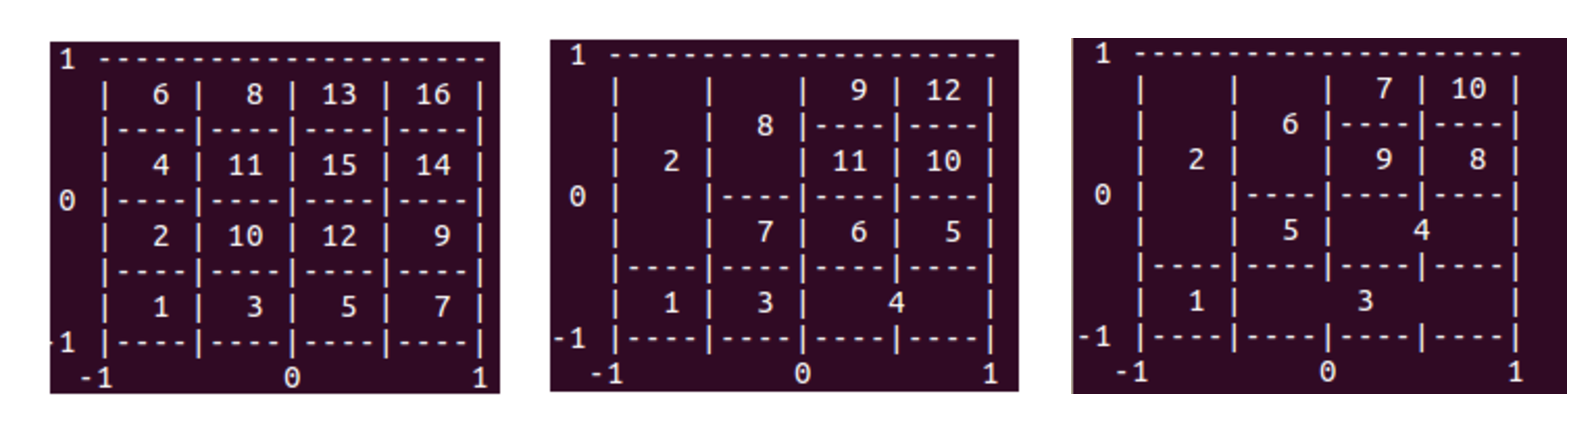
\includegraphics[width=\textwidth]{figures/bin_scheme.pdf} 
\caption{Binning combination scheme.}
\label{bins}
\end{figure}

The bins borders and the resulting cross section limits are shown in Tab.~\ref{bin_limits}:

\begin{table}[h!]
\centering
\begin{tabular}{llllllll}
Number of bins  & \multicolumn{6}{c}{Bin borders}  & Expected limit \\\hline 
                &$x_1$&$x_2$&$x_3$&$y_1$&$y_2$&$y_3$&\\\hline           
16 (default)    &-0.5 & 0.0 & 0.5 &-0.5 & 0.0 & 0.5 & $<2.91$\\
16              &-0.5 & 0.3 & 0.7 &-0.5 & 0.3 & 0.7 & $<2.83$\\
10              &-0.5 & 0.0 & 0.5 &-0.5 & 0.0 & 0.5 & $<2.93$\\
10              &-0.5 & 0.0 & 0.7 &-0.5 & 0.0 & 0.7 & $<2.86$\\
10              &-0.5 & 0.0 & 0.7 &-0.5 & 0.0 & 0.5 & $<2.84$\\
10              &-0.5 & 0.0 & 0.5 &-0.5 & 0.0 & 0.7 & $<2.87$\\
\textbf{10}     &\textbf{-0.5} &\textbf{ 0.4} &\textbf{ 0.7} &\textbf{-0.5} &\textbf{ 0.4} &\textbf{ 0.7} &$\mathbf{<2.81}$\\\hline
\end{tabular}
\caption{Limit variation as a function of bin size in the three lepton channel. (In bold: the final bin borders used in the analysis.)}
\label{bin_limits}
\end{table}


Combining the optimization of binning and using the tighter pre-selection cuts, the expected limit in the three lepton channel alone reaches $r<2.59$.

For same-sign dilepton channel, other binning combinations were also tested. 
First the three lepton binning was used to estimate the expected limit then bin borders were varied to obtain the best possible expected limit.
The bin borders and the resulting cross section limits for the same-sign dimuon channel are shown in Tab.~\ref{bin_limits_2lss}:

\begin{table}[h!]
\centering
\begin{tabular}{llllllll}
Number of bins  & \multicolumn{6}{c}{Bin borders}  & Expected limit \\\hline
                &$x_1$&$x_2$&$x_3$&$y_1$&$y_2$&$y_3$&\\\hline
16              &-0.5 & 0.4 & 0.7 &-0.5 & 0.4 & 0.7 & $<1.72$\\
12              &-0.5 & 0.4 & 0.7 &-0.5 & 0.4 & 0.7 & $<1.72$\\
12              &-0.3 & 0.4 & 0.7 &-0.5 & 0.4 & 0.7 & $<1.71$\\
12              &-0.3 & 0.3 & 0.7 &-0.5 & 0.4 & 0.7 & $<1.71$\\
12              &-0.3 & 0.3 & 0.7 &-0.4 & 0.4 & 0.7 & $<1.70$\\
12              &-0.3 & 0.3 & 0.7 &-0.3 & 0.4 & 0.7 & $<1.70$\\
12              &-0.3 & 0.3 & 0.7 &-0.3 & 0.2 & 0.7 & $<1.68$\\
12              &-0.3 & 0.3 & 0.7 &-0.3 & 0.1 & 0.7 & $<1.70$\\
12              &-0.3 & 0.3 & 0.7 &-0.3 & 0.2 & 0.6 & $<1.70$\\
10              &-0.5 & 0.4 & 0.7 &-0.5 & 0.4 & 0.7 & $<1.75$\\
\textbf{10}     &\textbf{-0.3} &\textbf{ 0.3} &\textbf{ 0.7} &\textbf{-0.3} &\textbf{ 0.2} &\textbf{ 0.6} &$\mathbf{<1.69}$\\\hline
\end{tabular}
\caption{Limit variation as a function of bin size in the same-sign dimuon channel. (In bold: the final bin borders used in the analysis.)}
\label{bin_limits_2lss}
\end{table}

The expected limit was found to be $r<1.69$ for optimized bin borders in 10 bins.


\subsection{Other binning strategies}
Two further strategies of clustering regions in the 2D plane of $BDT_{tt}$ vs $BDT_{ttV}$ into bins were attempted, following studies done in the \ttH\ multilepton analysis (and documented in greater detail in~\cite{CMS_AN_2017-029}).

\textbf{Clustering by S/B ratio}
The 2D plane is clustered into a given number of bins corresponding to regions where S/B is within a certain range.
The bin borders are determined such that the number of background events in each bin is approximately equal.
(See Sec.~5.3 in v4 of Ref.~\cite{CMS_AN_2017-029} for more details.)
The resulting regions for same-sign dilepton and three lepton events are shown in Fig.~\ref{fig:sbbinning}, with the expected distribution of signal and main backgrounds in Fig.~\ref{fig:sbfinalbins}.

\begin{figure} [!h]
 \centering
 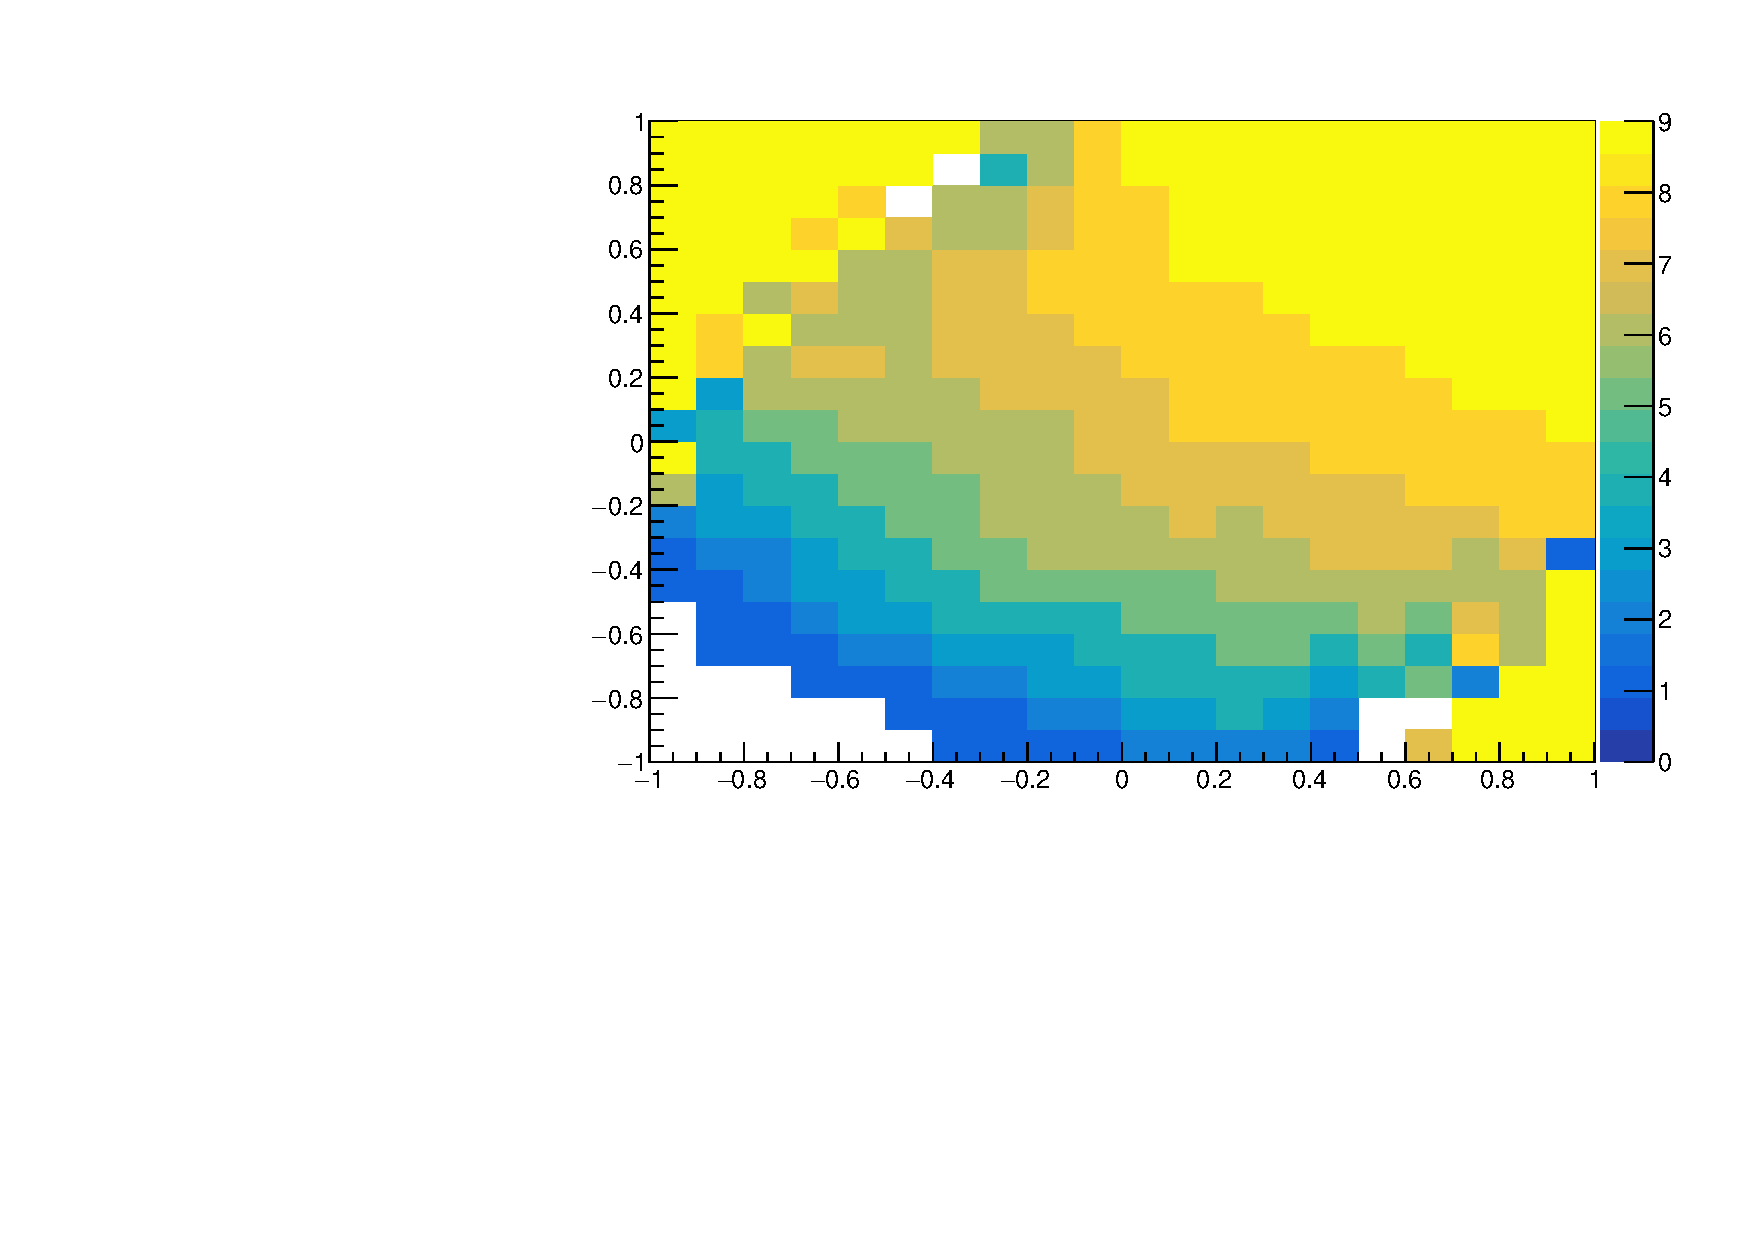
\includegraphics[width=0.45\textwidth]{figures/binning/hTargetBinning_2lss.pdf}
 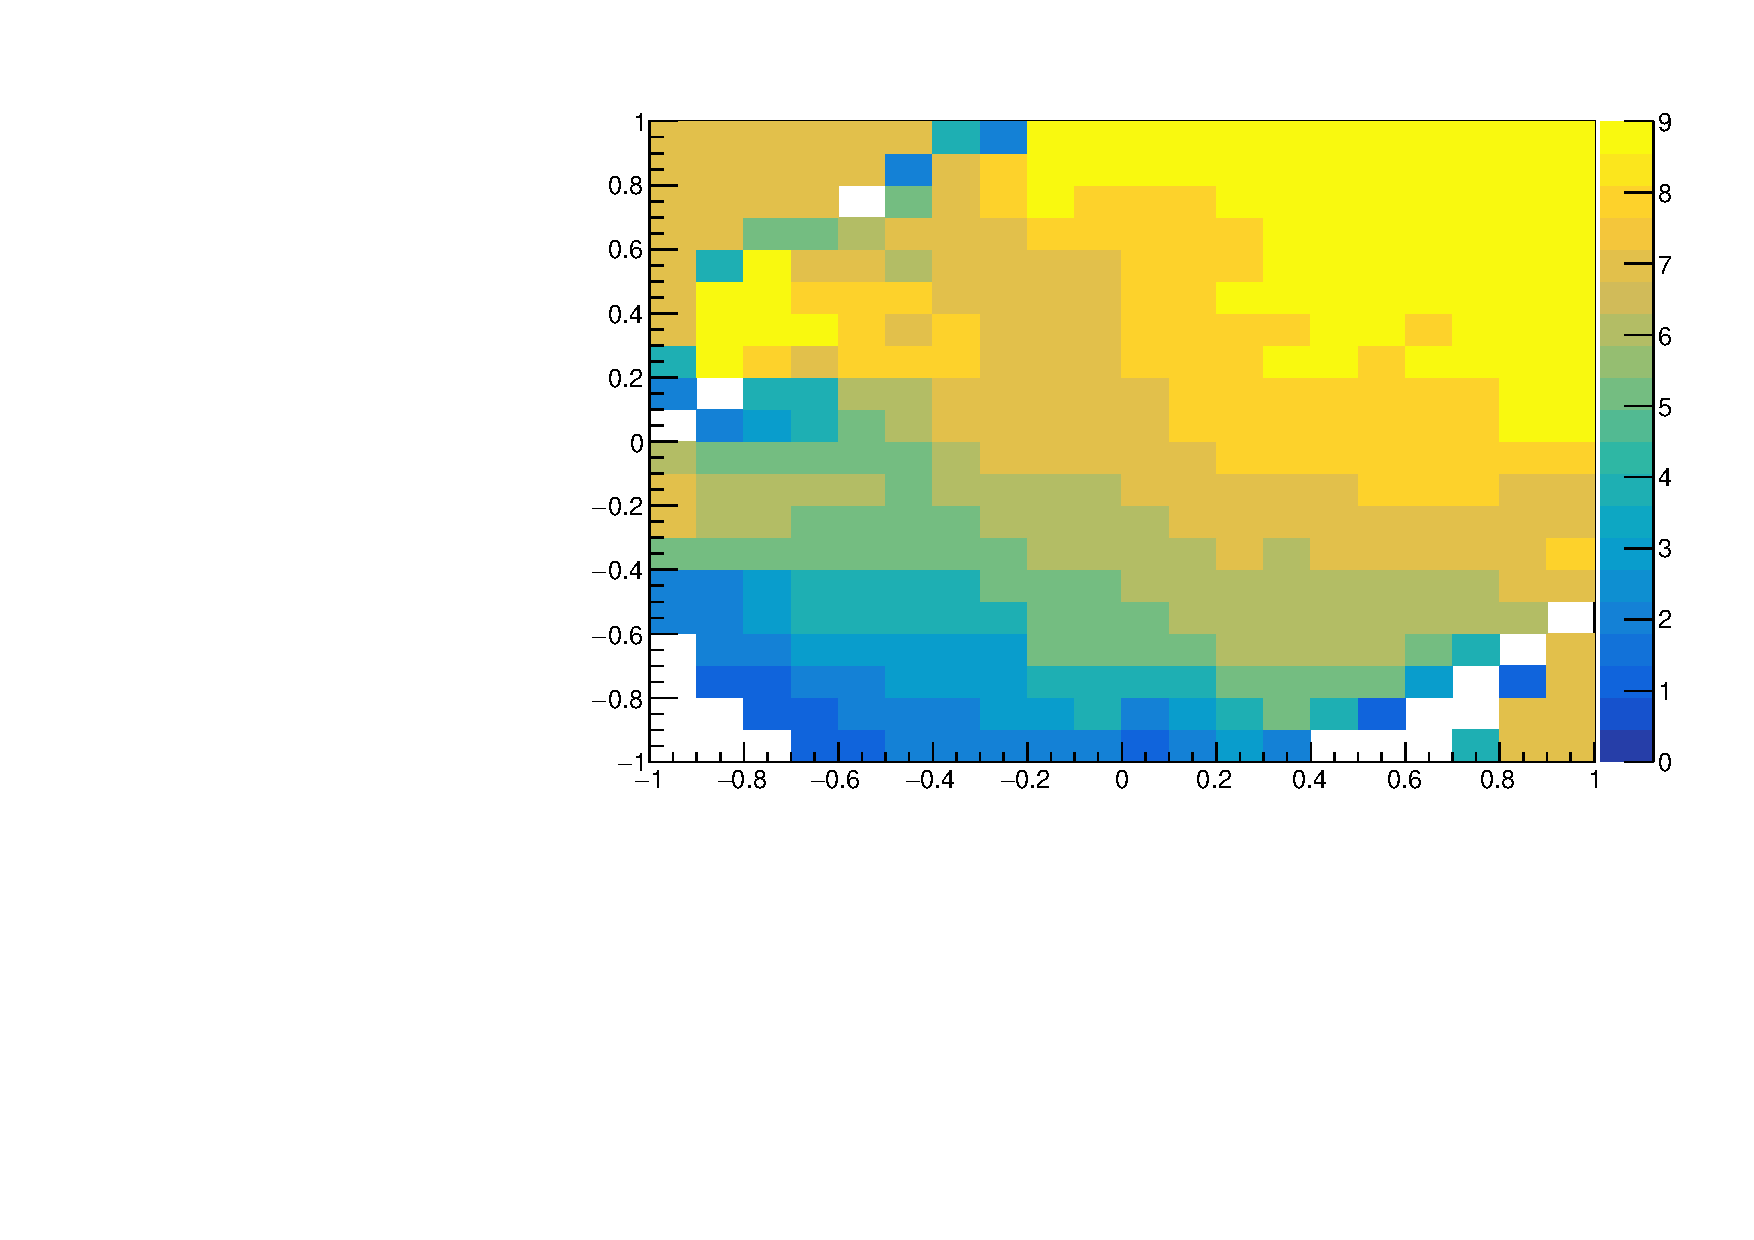
\includegraphics[width=0.45\textwidth]{figures/binning/hTargetBinning_3l.pdf}
\caption{Binning by S/B regions for same-sign dilepton (left) and three leptons (right).}
\label{fig:sbbinning}
\end{figure}

\begin{figure} [!h]
 \centering
 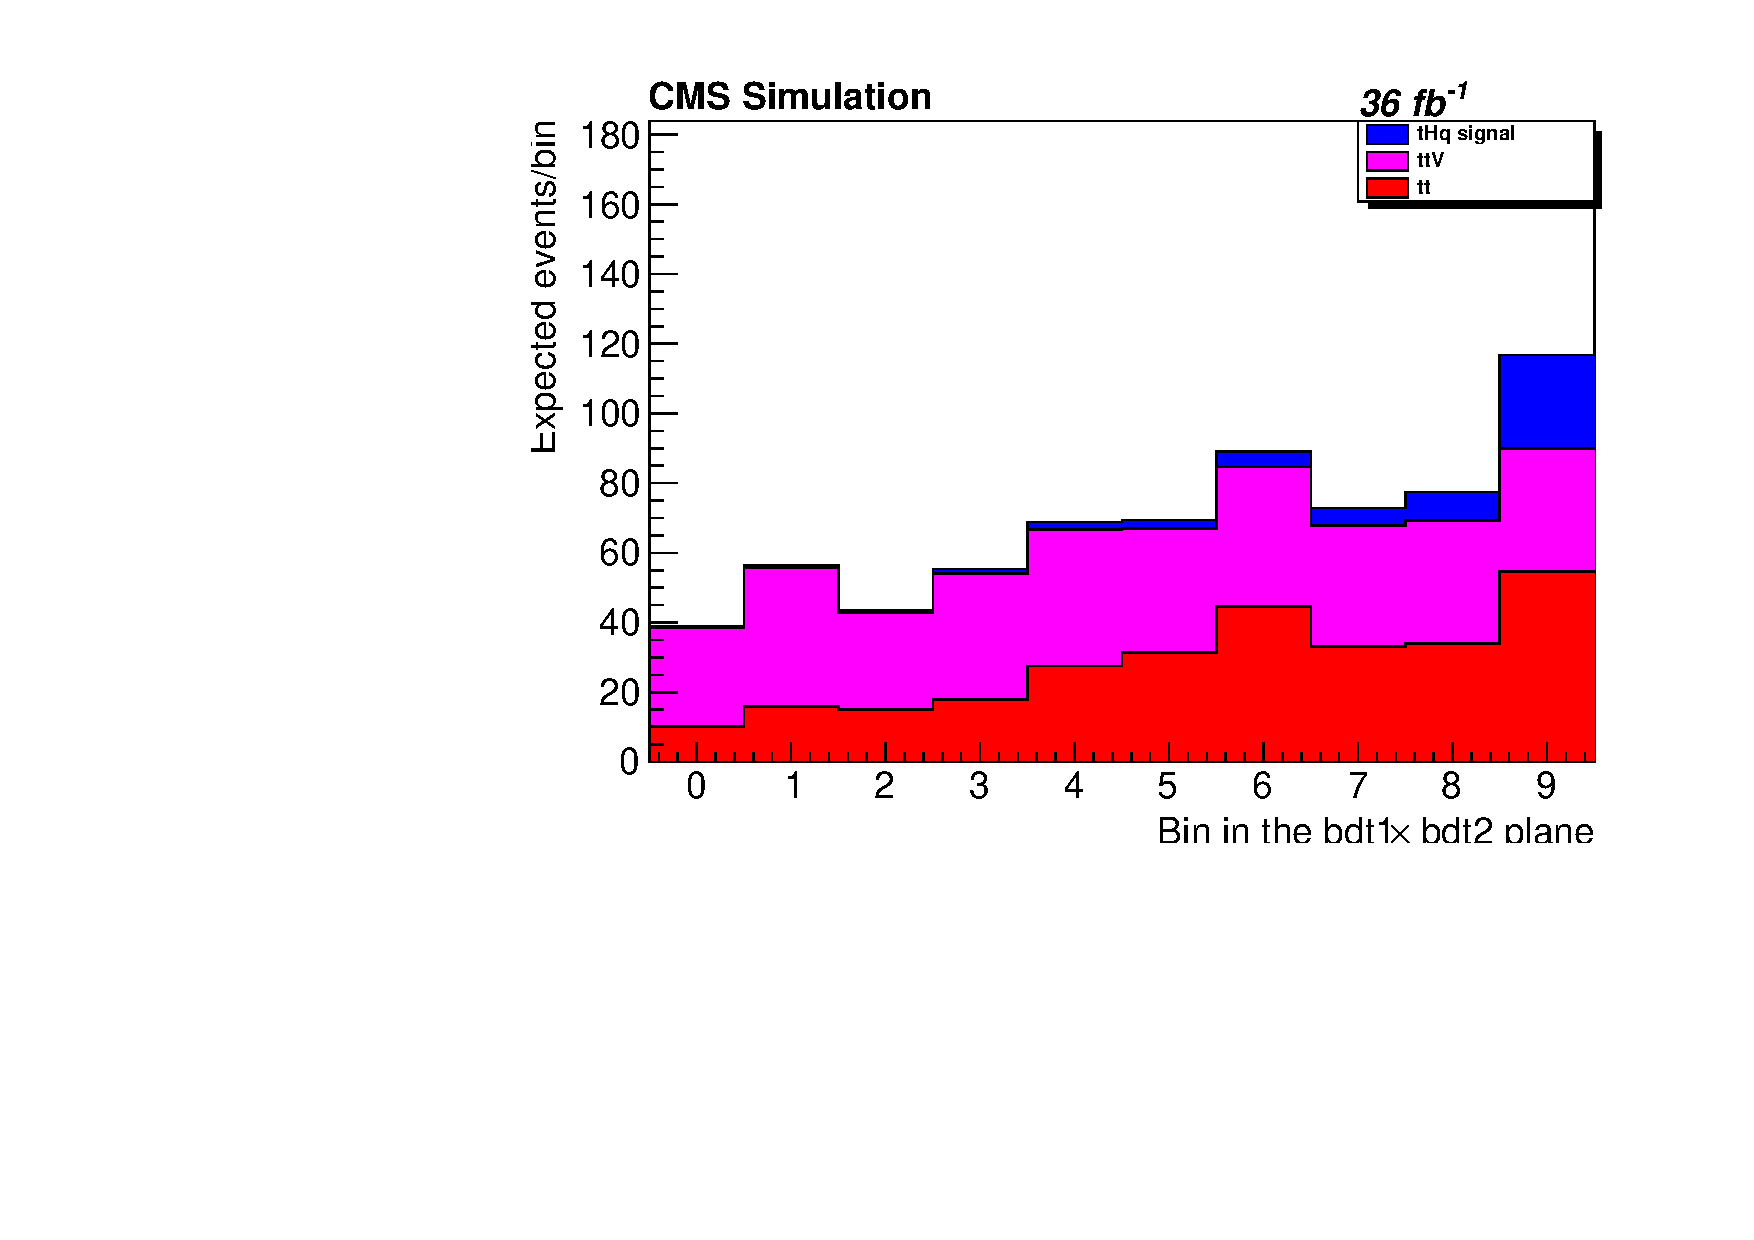
\includegraphics[width=0.45\textwidth]{figures/binning/likelihoodBased_1d_2lss.pdf}
 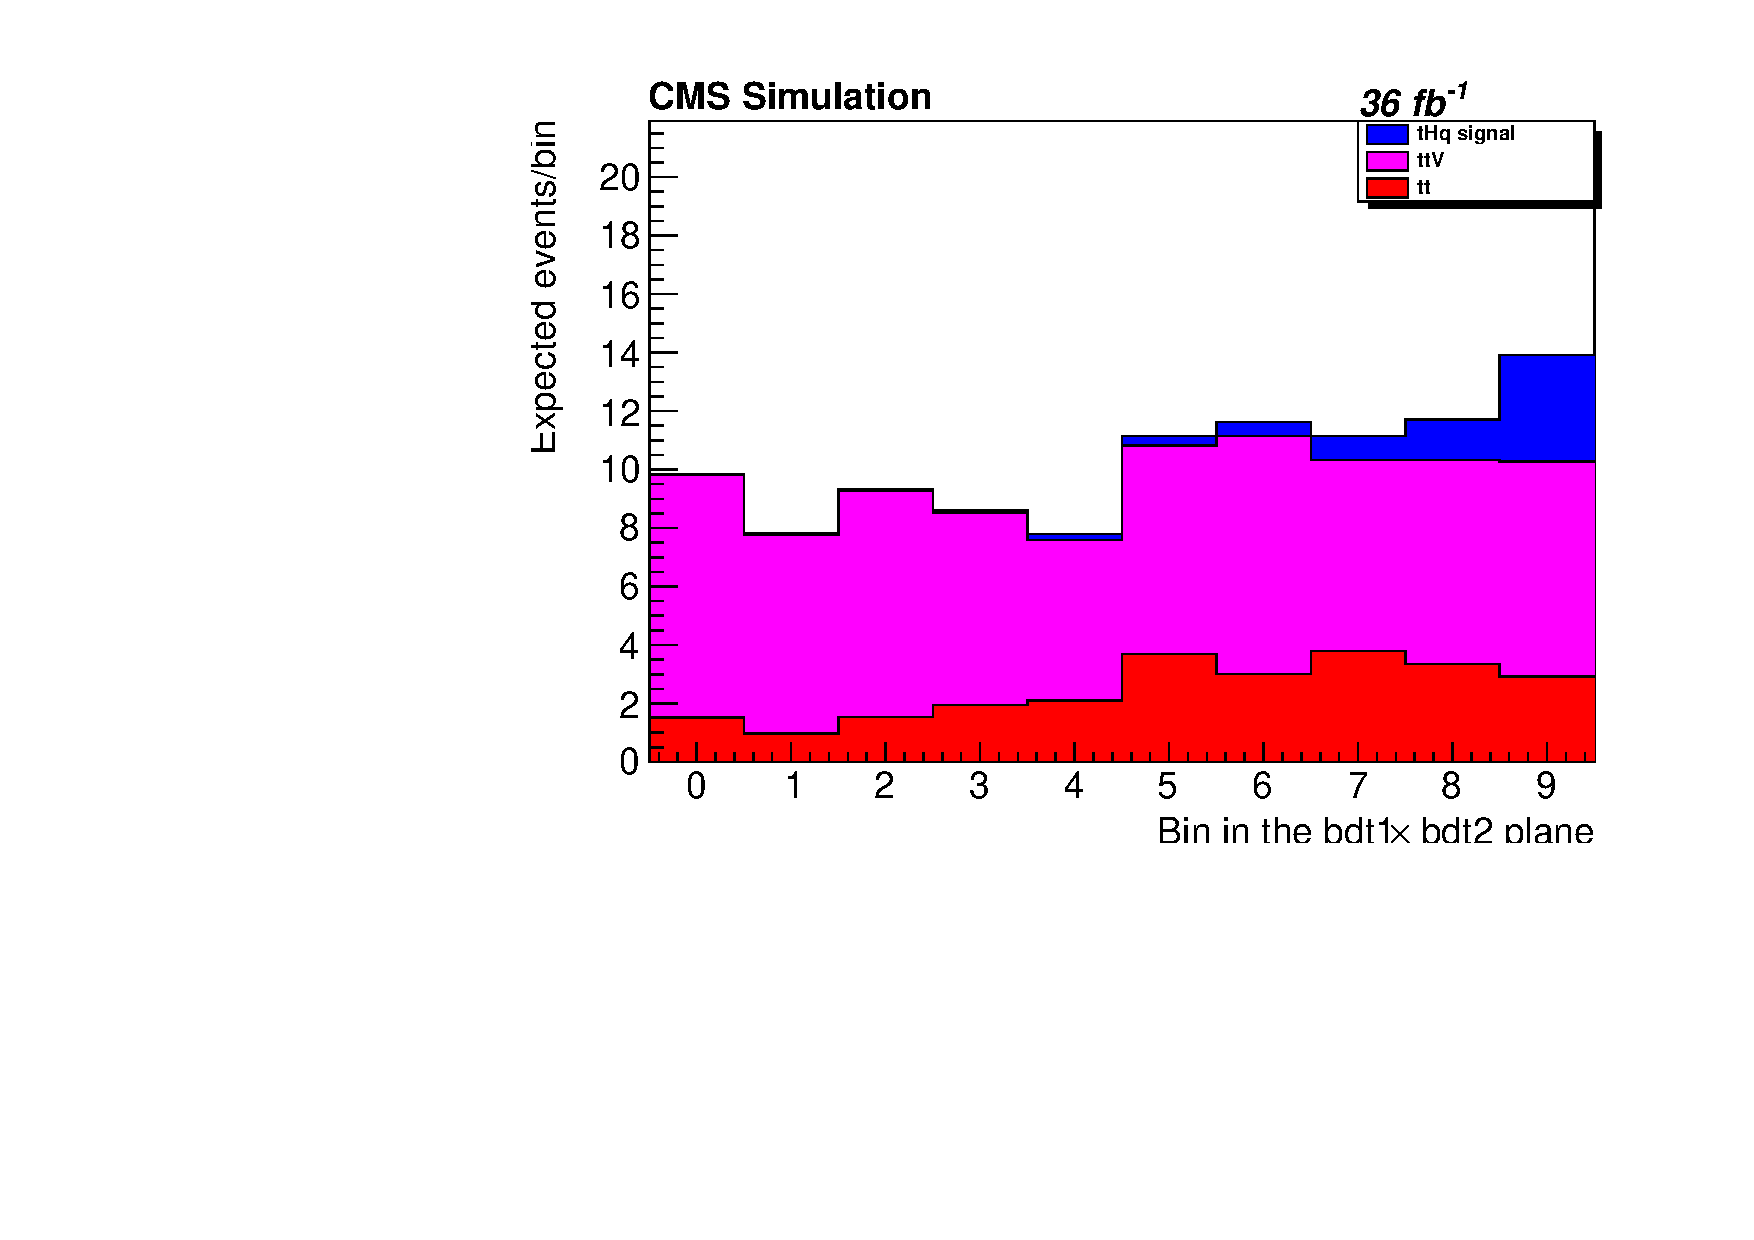
\includegraphics[width=0.45\textwidth]{figures/binning/likelihoodBased_1d_3l.pdf}
\caption{Final bins (corresponding to S/B regions in the 2D plane) for same-sign dilepton (left) and three leptons (right).}
\label{fig:sbfinalbins}
\end{figure}

Using this technique, the resulting limits (for the $\Ct=-1, \CV=1$ scenario) are about 20\% worse than with the binnings described above: \mumu\ changed from 1.82 to 2.15, \threel\ from 1.52 to 1.75.

\textbf{$k$-Means geometric clustering}
A second clustering strategy employs a recursive application of the $k$-means algorithm (see Appendix D in v4 of Ref.~\cite{CMS_AN_2017-029}) to separate the 2D plane into geometric regions.
The resulting clustering (using the \ttH\ multilepton code on \tHq\ signal and \ttbar\ and \ttV\ background events) are shown in Fig.~\ref{fig:kmeansbinning}.
The expected distribution of events for the signal and main background in these bins is shown in Fig.~\ref{fig:kmeansfinalbins}.
\begin{figure} [!h]
 \centering
 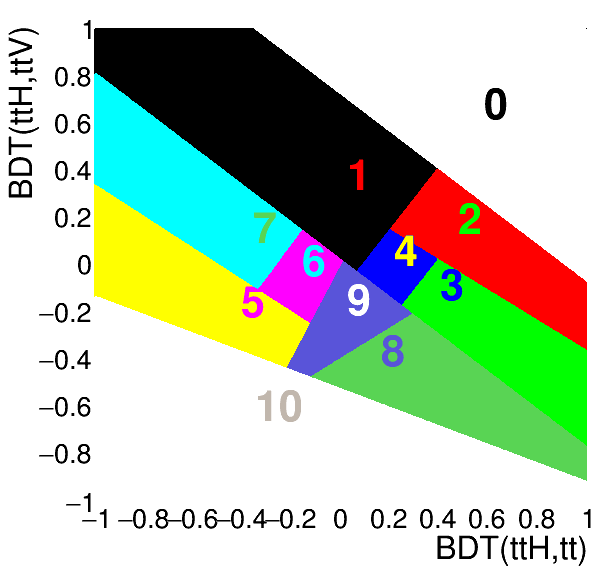
\includegraphics[width=0.45\textwidth]{figures/binning/voronoi_2l_trial0.png}
 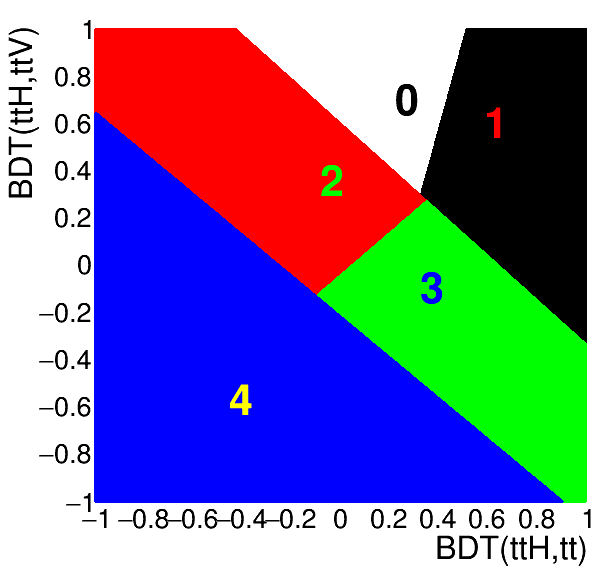
\includegraphics[width=0.45\textwidth]{figures/binning/voronoi_3l_trial0.png}
\caption{Binning into geometric regions using a $k$-means algorithm for same-sign dilepton (left) and three leptons (right).}
\label{fig:kmeansbinning}
\end{figure}

\begin{figure} [!h]
 \centering
 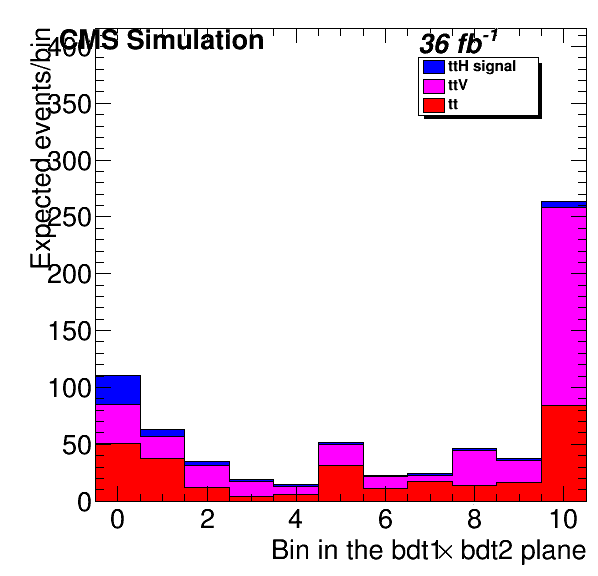
\includegraphics[width=0.45\textwidth]{figures/binning/recursiveNoOrdering_2l_trial0.png}
 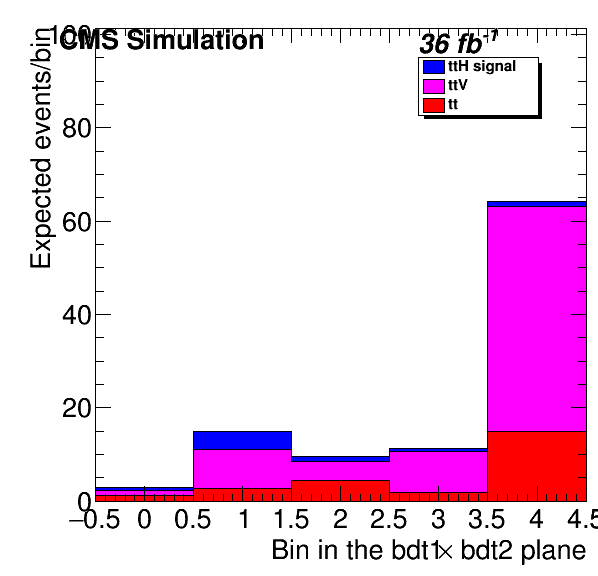
\includegraphics[width=0.45\textwidth]{figures/binning/recursiveNoOrdering_3l_trial0.png}
\caption{Final bins using a $k$-means algorithm for same-sign dilepton (left) and three leptons (right). Note that the bin numbering here is such that signal-like bins are lower.}
\label{fig:kmeansfinalbins}
\end{figure}

Similarly to the S/B ratio binning, the limits using the $k$-means clustering are significantly worse than those of the bins described before.
In the \mumu\ channel, the limit deteriorates from 1.82 to 2.05, whereas in \threel\ it changes from 1.58 to 1.78.
